\documentclass[aspectratio=169,11pt]{beamer}

\usetheme{metropolis}
\usepackage{booktabs}
\usepackage{graphicx}
\usepackage{tikz}
\usetikzlibrary{positioning}
\usepackage{amsmath,amssymb}
\usepackage{listings}
\usepackage{xcolor}
\usepackage{hyperref}
\usepackage{multicol}

\definecolor{columbiaBlue}{HTML}{185494}
\definecolor{accentOrange}{HTML}{E87722}
\definecolor{lightGray}{HTML}{F5F5F5}
\definecolor{codeGreen}{HTML}{2E7D32}

\setbeamercolor{frametitle}{bg=columbiaBlue,fg=white}
\setbeamercolor{progress bar}{fg=accentOrange}
\setbeamercolor{alerted text}{fg=accentOrange}

\lstset{
  basicstyle=\ttfamily\scriptsize,
  keywordstyle=\color{columbiaBlue},
  commentstyle=\color{gray},
  stringstyle=\color{codeGreen},
  breaklines=true,
  frame=single,
  backgroundcolor=\color{lightGray},
}

% ---- Reusable callout for data-type connections ----
\newcommand{\datatypebox}[1]{%
  \par\vspace{0.15em}%
  \noindent\colorbox{columbiaBlue!10}{\parbox{\dimexpr\linewidth-2\fboxsep}{%
    \footnotesize\textcolor{columbiaBlue}{\textbf{Data type connection:}} #1}}%
}

\title{Lecture 19: Clinical \& Biomedical Text}
\subtitle{Data Modalities}
\author{BINF 4002 --- Machine Learning for Health}
\date{Tuesday, March 31, 2026}
\institute{Columbia University Irving Medical Center}

\begin{document}

% ============================================================
\begin{frame}[plain,noframenumbering]
\vspace*{-1.2em}
\titlepage
\end{frame}

% ============================================================
\begin{frame}{Where Are We?}
\begin{columns}[T]
\begin{column}{0.55\textwidth}
Lectures 17--18: EHR data is a \textbf{byproduct of clinical care and billing}. A patient's record is a timeline of multi-modal observations.

\vspace{0.3em}
\textbf{Today:} We zoom into the \textbf{text} on that timeline --- the richest, messiest, and most rapidly changing part of the EHR.

\pause
\vspace{0.3em}
\textbf{Running thread:} Text is a \emph{sequence of nominal tokens}. We'll see \textbf{five ways} clinical text breaks that abstraction. Watch for the \colorbox{columbiaBlue!10}{\textcolor{columbiaBlue}{\textbf{Data type connection}}} boxes.

\vspace{0.2em}
{\small Notebook: \texttt{nb19\_clinical\_text\_data.ipynb}}
\end{column}
\begin{column}{0.43\textwidth}
\centering
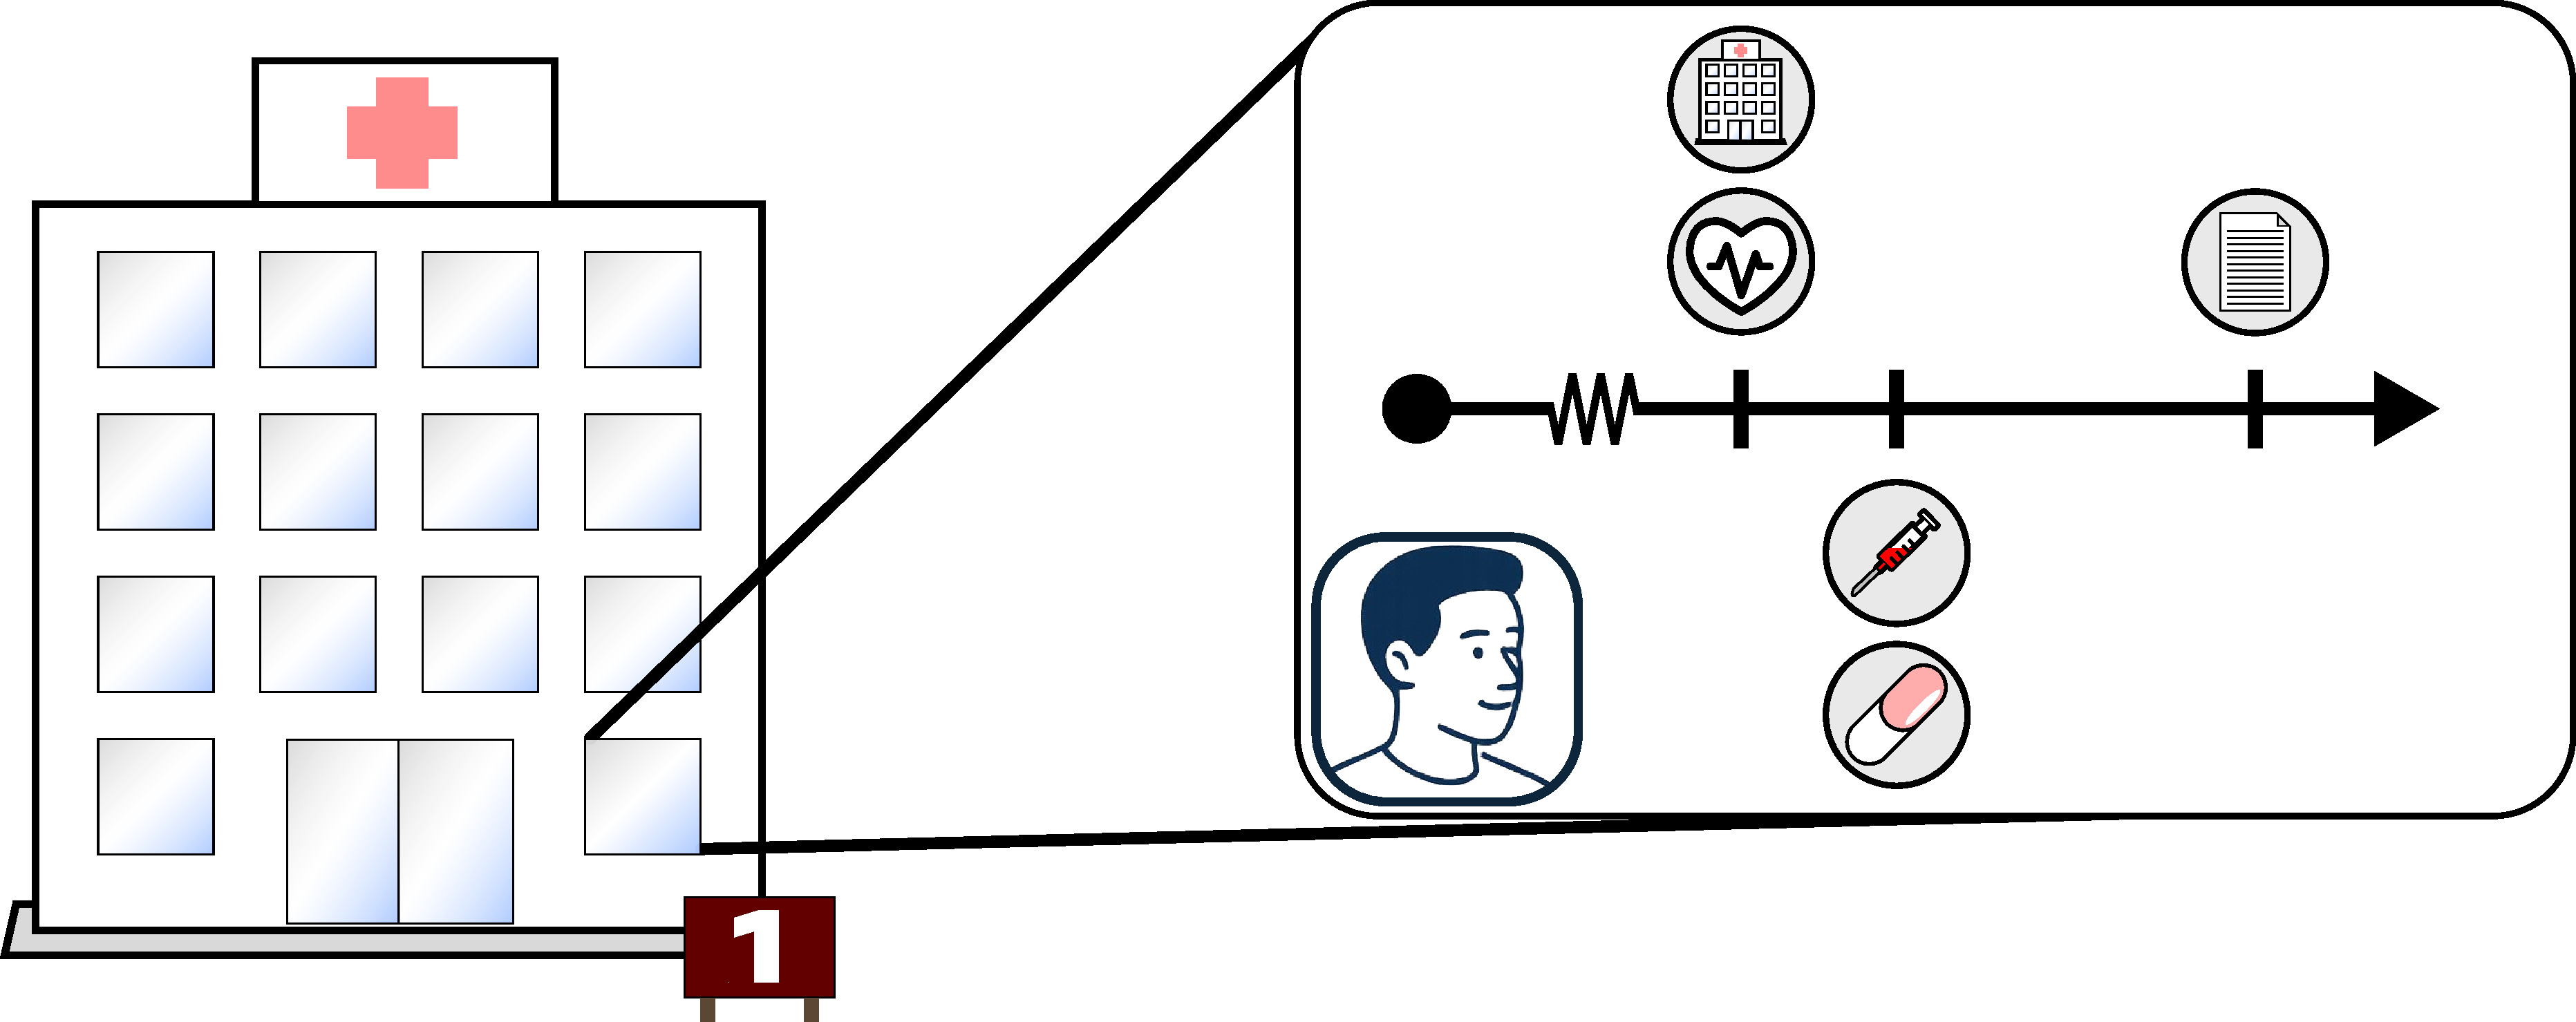
\includegraphics[width=\linewidth,height=4.5cm,keepaspectratio]{figures/fig19_timeline_with_note.pdf}
\end{column}
\end{columns}
\end{frame}

% ============================================================
\section{A Paradox to Keep in Mind}

% ============================================================
\begin{frame}{A Puzzle from 1865}
\textbf{England, 1860s.} Steam engines are getting more efficient every decade.

\vspace{0.3em}
\begin{center}
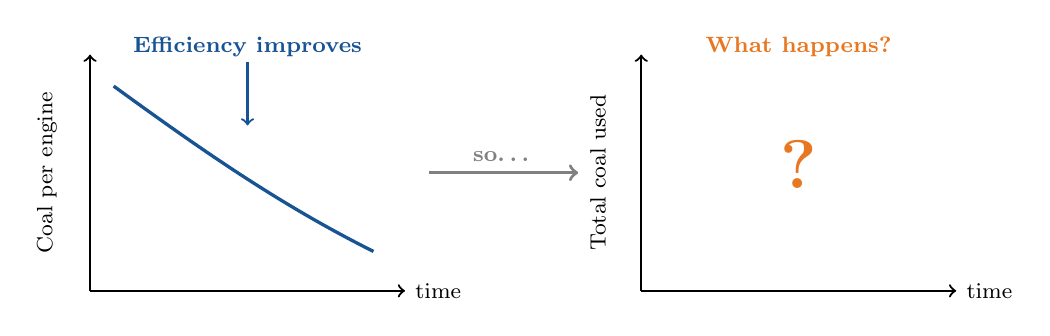
\begin{tikzpicture}[font=\small]
  % Left graph: coal per engine going down
  \begin{scope}[shift={(0,0)}]
    \draw[->, thick] (0,0) -- (4.0,0) node[right, font=\footnotesize] {time};
    \draw[->, thick] (0,0) -- (0,3.0);
    \node[rotate=90, font=\footnotesize] at (-0.55,1.5) {Coal per engine};
    \draw[very thick, columbiaBlue] (0.3,2.6) .. controls (1.4,1.8) and (2.4,1.1) .. (3.6,0.5);
    \node[font=\footnotesize\bfseries, columbiaBlue] at (2.0,3.1) {Efficiency improves};
    \draw[->, columbiaBlue, thick] (2.0,2.9) -- (2.0,2.1);
  \end{scope}
  % Arrow between
  \draw[->, very thick, gray] (4.3,1.5) -- (6.2,1.5) node[midway, above, font=\footnotesize\bfseries] {so\ldots};
  % Right graph: total coal = ???
  \begin{scope}[shift={(7.0,0)}]
    \draw[->, thick] (0,0) -- (4.0,0) node[right, font=\footnotesize] {time};
    \draw[->, thick] (0,0) -- (0,3.0);
    \node[rotate=90, font=\footnotesize] at (-0.55,1.5) {Total coal used};
    \node[font=\Huge\bfseries, accentOrange] at (2.0,1.6) {?};
    \node[font=\footnotesize\bfseries, accentOrange] at (2.0,3.1) {What happens?};
  \end{scope}
\end{tikzpicture}
\end{center}

\vspace{0.3em}
Each engine uses \emph{less} coal. Surely total coal consumption goes \emph{down}?
\end{frame}

% ============================================================
\begin{frame}{The Jevons Paradox}
\small
\textbf{Jevons} (1865) discovered the answer was \emph{counterintuitive}:

\vspace{0.15em}
\begin{center}
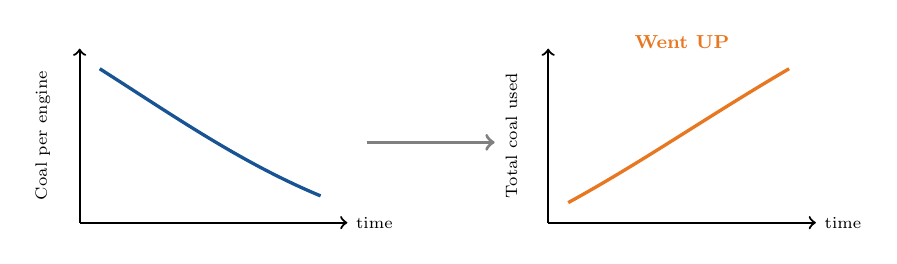
\begin{tikzpicture}[font=\scriptsize, scale=0.85, every node/.style={scale=0.85}]
  \begin{scope}[shift={(0,0)}]
    \draw[->, thick] (0,0) -- (4.0,0) node[right] {time};
    \draw[->, thick] (0,0) -- (0,2.6);
    \node[rotate=90] at (-0.55,1.3) {Coal per engine};
    \draw[very thick, columbiaBlue] (0.3,2.3) .. controls (1.4,1.6) and (2.4,0.9) .. (3.6,0.4);
  \end{scope}
  \draw[->, very thick, gray] (4.3,1.2) -- (6.2,1.2);
  \begin{scope}[shift={(7.0,0)}]
    \draw[->, thick] (0,0) -- (4.0,0) node[right] {time};
    \draw[->, thick] (0,0) -- (0,2.6);
    \node[rotate=90] at (-0.55,1.3) {Total coal used};
    \draw[very thick, accentOrange] (0.3,0.3) .. controls (1.4,0.9) and (2.4,1.6) .. (3.6,2.3);
    \node[font=\footnotesize\bfseries, accentOrange] at (2.0,2.7) {Went \textbf{UP}};
  \end{scope}
\end{tikzpicture}
\end{center}

\pause
\vspace{0.1em}
Efficiency made coal-powered activity \emph{cheaper}, so people did \textbf{far more of it}. Total consumption rose.

\pause
\vspace{0.1em}
\textbf{The Jevons Paradox:} Making something easier to produce often yields \emph{more} of it, not less effort overall. \textbf{Keep this in mind} as we tour clinical text.
\end{frame}

% ============================================================
\section{Who Writes Health Text, For Whom, and Why?}

% ============================================================
\begin{frame}{A Taxonomy of Health Text by Communicative Purpose}
Health text is not one thing. Four broad categories:

\vspace{0.15em}
\begin{center}
\scriptsize
\renewcommand{\arraystretch}{1.05}
\begin{tabular}{llp{2.3cm}p{3.0cm}}
\toprule
\textbf{Category} & \textbf{Writer $\to$ Reader} & \textbf{Purpose} & \textbf{Examples} \\
\midrule
Clinical documentation & Clinician $\to$ Record & Legal, billing, continuity & Progress notes, H\&Ps, discharge sums \\
Clinical communication & Clinician $\to$ Clinician/Patient & Handoff, referral & Rad/path reports, consults, AVS \\
Patient-generated & Patient $\to$ World/Clinician & Help-seeking & Portal messages, forums, social media \\
Scientific literature & Researcher $\to$ Researcher & Knowledge creation & PubMed, PMC, textbooks \\
\bottomrule
\end{tabular}
\end{center}

\pause
\vspace{0.15em}
{\footnotesize Not exhaustive --- also regulatory text, insurance narratives, public health reports. But these four cover most of what ML researchers encounter. We'll take them in order.}
\end{frame}

% ============================================================
\section{Clinical Documentation}

% ============================================================
\begin{frame}{What Is Clinical Documentation?}
\textbf{Clinical documentation} = the notes clinicians write to record what happened during a patient encounter.

\pause
\vspace{0.3em}
Three simultaneous purposes, often in tension:
\begin{itemize}[<+->]\setlength\itemsep{0.1em}
  \item \textbf{Billing:} Justify reimbursement via E\&M coding (how thorough was the visit?).
  \item \textbf{Legal protection:} ``If it wasn't documented, it didn't happen.''
  \item \textbf{Care continuity:} Communicate the patient's story to the next clinician.
\end{itemize}

\onslide<5->{
\vspace{0.2em}
\alert{Key framing:} Everything that follows --- templates, copy-paste, abbreviations --- is a \textbf{rational response} to writing notes that must serve all three purposes under extreme time pressure.

\vspace{0.1em}
{\small [Notebook Cell~3: loads MTSamples, $\sim$5K clinical transcriptions across 40 specialties.]}}
\end{frame}

% ============================================================
\begin{frame}{Who Writes Clinical Notes, and Under What Conditions?}
\textbf{Recall from Lecture 17:} EHR data reflects what was \emph{documented}, not everything that \emph{happened}.

\vspace{0.3em}
\textbf{The clinician's reality:}
\begin{itemize}[<+->]\setlength\itemsep{0.05em}
  \item US physicians spend \textbf{$\sim$2 hours on documentation for every 1 hour of patient contact} (Sinsky et al., 2016).
  \item ``Pajama time'': charting after hours, evenings, weekends.
  \item Notes must satisfy billing, legal, \emph{and} clinical needs --- often in tension.
  \item Time pressure leads to shortcuts: templates, copy-paste, abbreviations.
\end{itemize}
\end{frame}

% ============================================================
\begin{frame}{Who Generates What? A Cast of Authors}
``Clinical notes'' are not all written by the same person:

\vspace{0.15em}
\begin{center}
\scriptsize
\renewcommand{\arraystretch}{1.0}
\begin{tabular}{lp{3.5cm}p{5.0cm}}
\toprule
\textbf{Author} & \textbf{Typical notes} & \textbf{Characteristics} \\
\midrule
Attending physician & H\&Ps, progress notes, discharge summaries & Most autonomy; may dictate or use scribe \\
Resident / fellow & Same, co-signed by attending & Learning; notes often more verbose \\
Nurse / RN & Nursing assessments, flowsheets, triage & Frequent, structured, shift-based \\
APP (NP/PA) & Progress notes, procedure notes & Similar to physician; scope varies by state \\
SW, PT, OT, dietitian & Discipline-specific assessments & Different vocabulary and templates \\
\bottomrule
\end{tabular}
\end{center}

\pause
\vspace{0.1em}
\alert{For ML:} Author identity may or may not be in your dataset. Note style, vocabulary, and length vary \emph{systematically} by role --- an unobserved confounder if you ignore it.
\end{frame}

% ============================================================
\begin{frame}{The Template--Free-Text Hybrid}
\begin{columns}[T]
\begin{column}{0.48\textwidth}
\centering
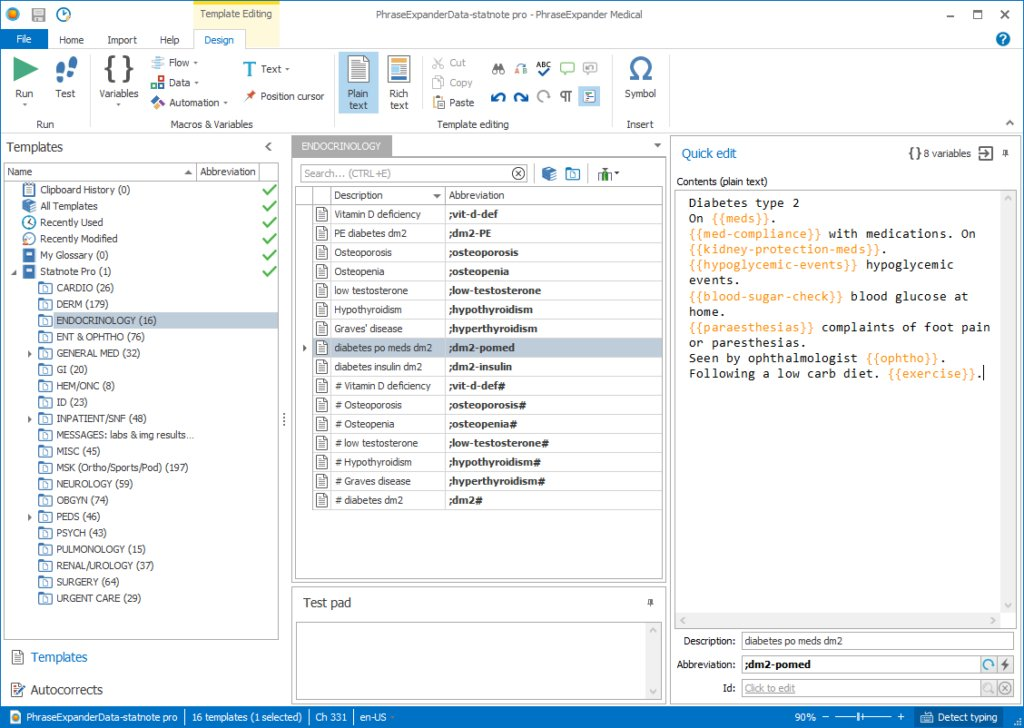
\includegraphics[width=\linewidth,height=2.8cm,keepaspectratio]{figures/fig19_template_phraseexpander.png}\\[1pt]
{\scriptsize \textbf{(a)} Template expansion: \texttt{;dm2-pomed} generates a full diabetes note with variables.}
\end{column}
\begin{column}{0.48\textwidth}
\centering
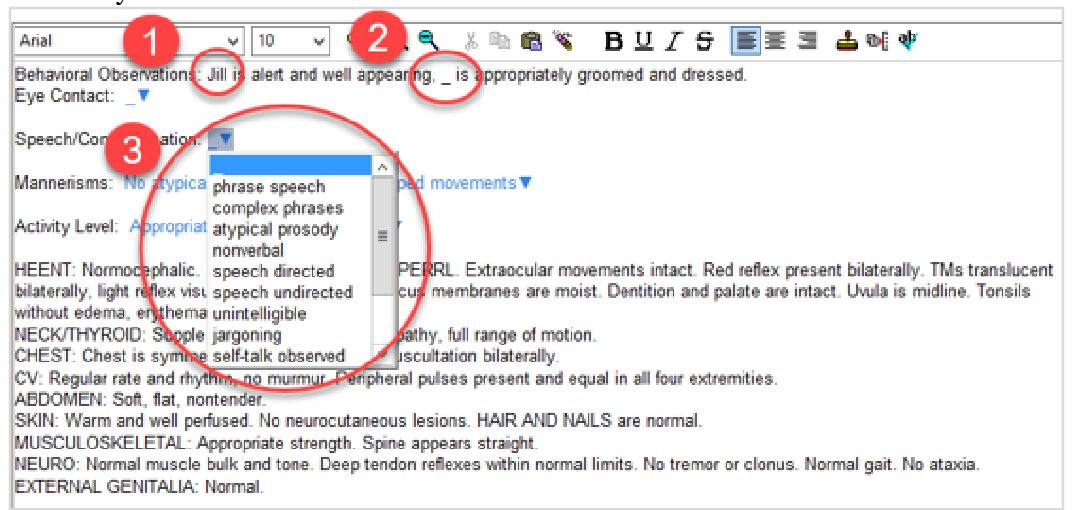
\includegraphics[width=\linewidth,height=2.8cm,keepaspectratio]{figures/fig19_template_ehr_dropdowns.png}\\[1pt]
{\scriptsize \textbf{(b)} EHR template: dropdowns constrain input to pre-defined options.}
\end{column}
\end{columns}

\vspace{0.1em}
\small
\textbf{Result:} Most ``text'' in a clinical note is \textbf{machine-generated boilerplate}. The clinician's actual reasoning is often just 1--2 sentences in the Assessment \& Plan.

\pause
\vspace{0.05em}
\alert{Key implication:} An LLM trained on clinical notes is partly learning to emulate \textbf{template engines and copy-paste} --- generative processes that were already automated \emph{before} any ML entered.
\end{frame}

% ============================================================
\begin{frame}{How Much Variation? Note Length by Specialty}
\begin{center}
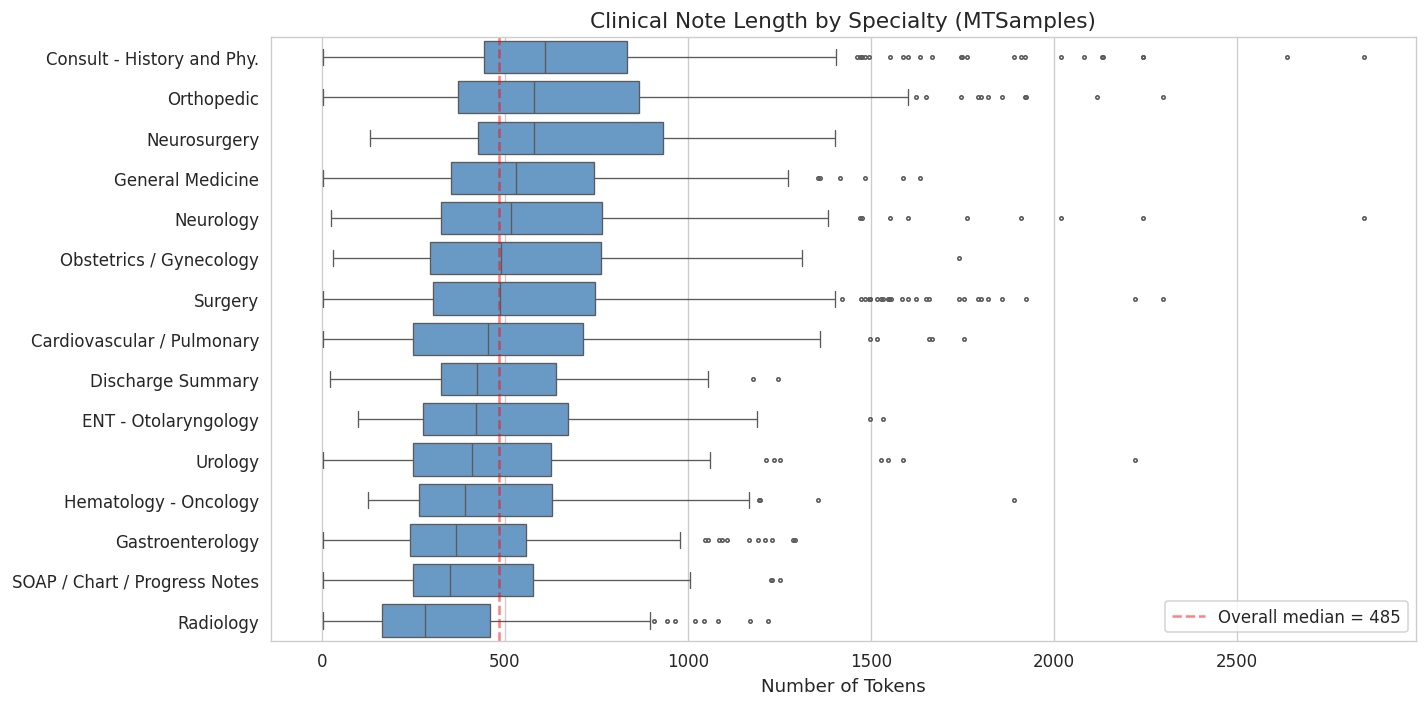
\includegraphics[width=0.88\linewidth,height=0.65\textheight,keepaspectratio]{figures/fig19_1_note_length.png}
\end{center}

\vspace{-0.3em}
\small
Discharge summaries and surgical notes can be 10$\times$ longer than radiology reports. ``Clinical text'' is not one distribution --- it's many. {\footnotesize [Notebook Cell~4]}
\end{frame}

% ============================================================
\begin{frame}{Copy-Paste \& Note Bloat}
Studies estimate \textbf{50--80\%} of text in clinical notes is duplicated from prior notes or templates (Tsou et al., 2017; Cohen et al., 2013).

\vspace{0.2em}
\textbf{Why this matters for ML:}
\begin{itemize}[<+->]\setlength\itemsep{0.08em}
  \item \textbf{Information content $\neq$ text volume.} A 10-page note may contain 1 page of new information.
  \item Na\"ive models treat every token equally $\Rightarrow$ dominated by boilerplate signal.
  \item Copy-pasted text creates \textbf{train--test leakage} if you split by note instead of patient.
\end{itemize}

\onslide<4->{\datatypebox{Each note is part of a \textbf{temporal sequence} of notes for the same patient. Copy-paste means successive tokens are \textbf{not i.i.d.}\ --- 70\% duplication shatters the independence assumption.}}
\end{frame}

% ============================================================
\begin{frame}{Copy-Paste Evidence: Between-Patient Template Overlap}
\begin{center}
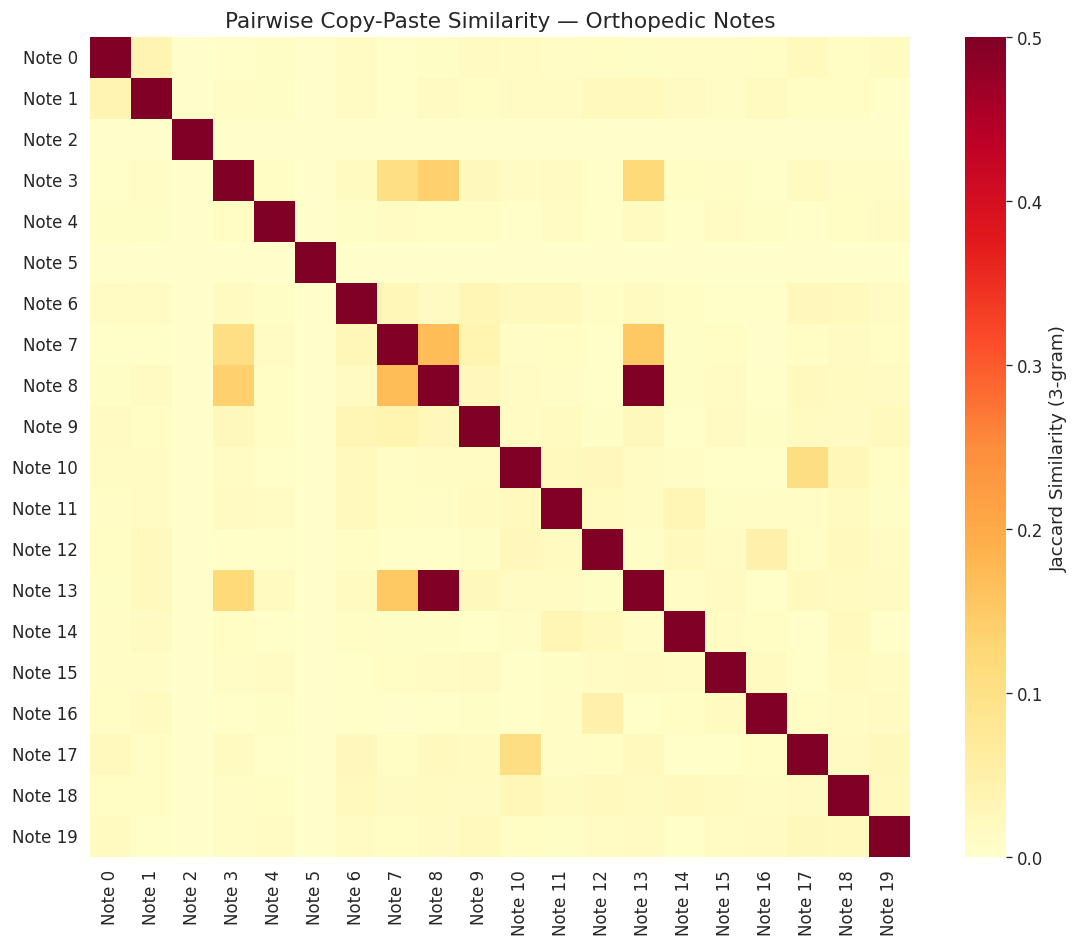
\includegraphics[width=0.62\linewidth,height=0.60\textheight,keepaspectratio]{figures/fig19_3_copypaste_heatmap.png}
\end{center}

\vspace{-0.3em}
\small
Pairwise Jaccard similarity within one specialty. MTSamples lacks longitudinal patient data, so this is \emph{between-patient template overlap} --- real EHR within-patient overlap would be much higher. {\footnotesize [Notebook Cell~6]}
\end{frame}

% ============================================================
\begin{frame}{Text in the Patient Timeline}
\begin{center}
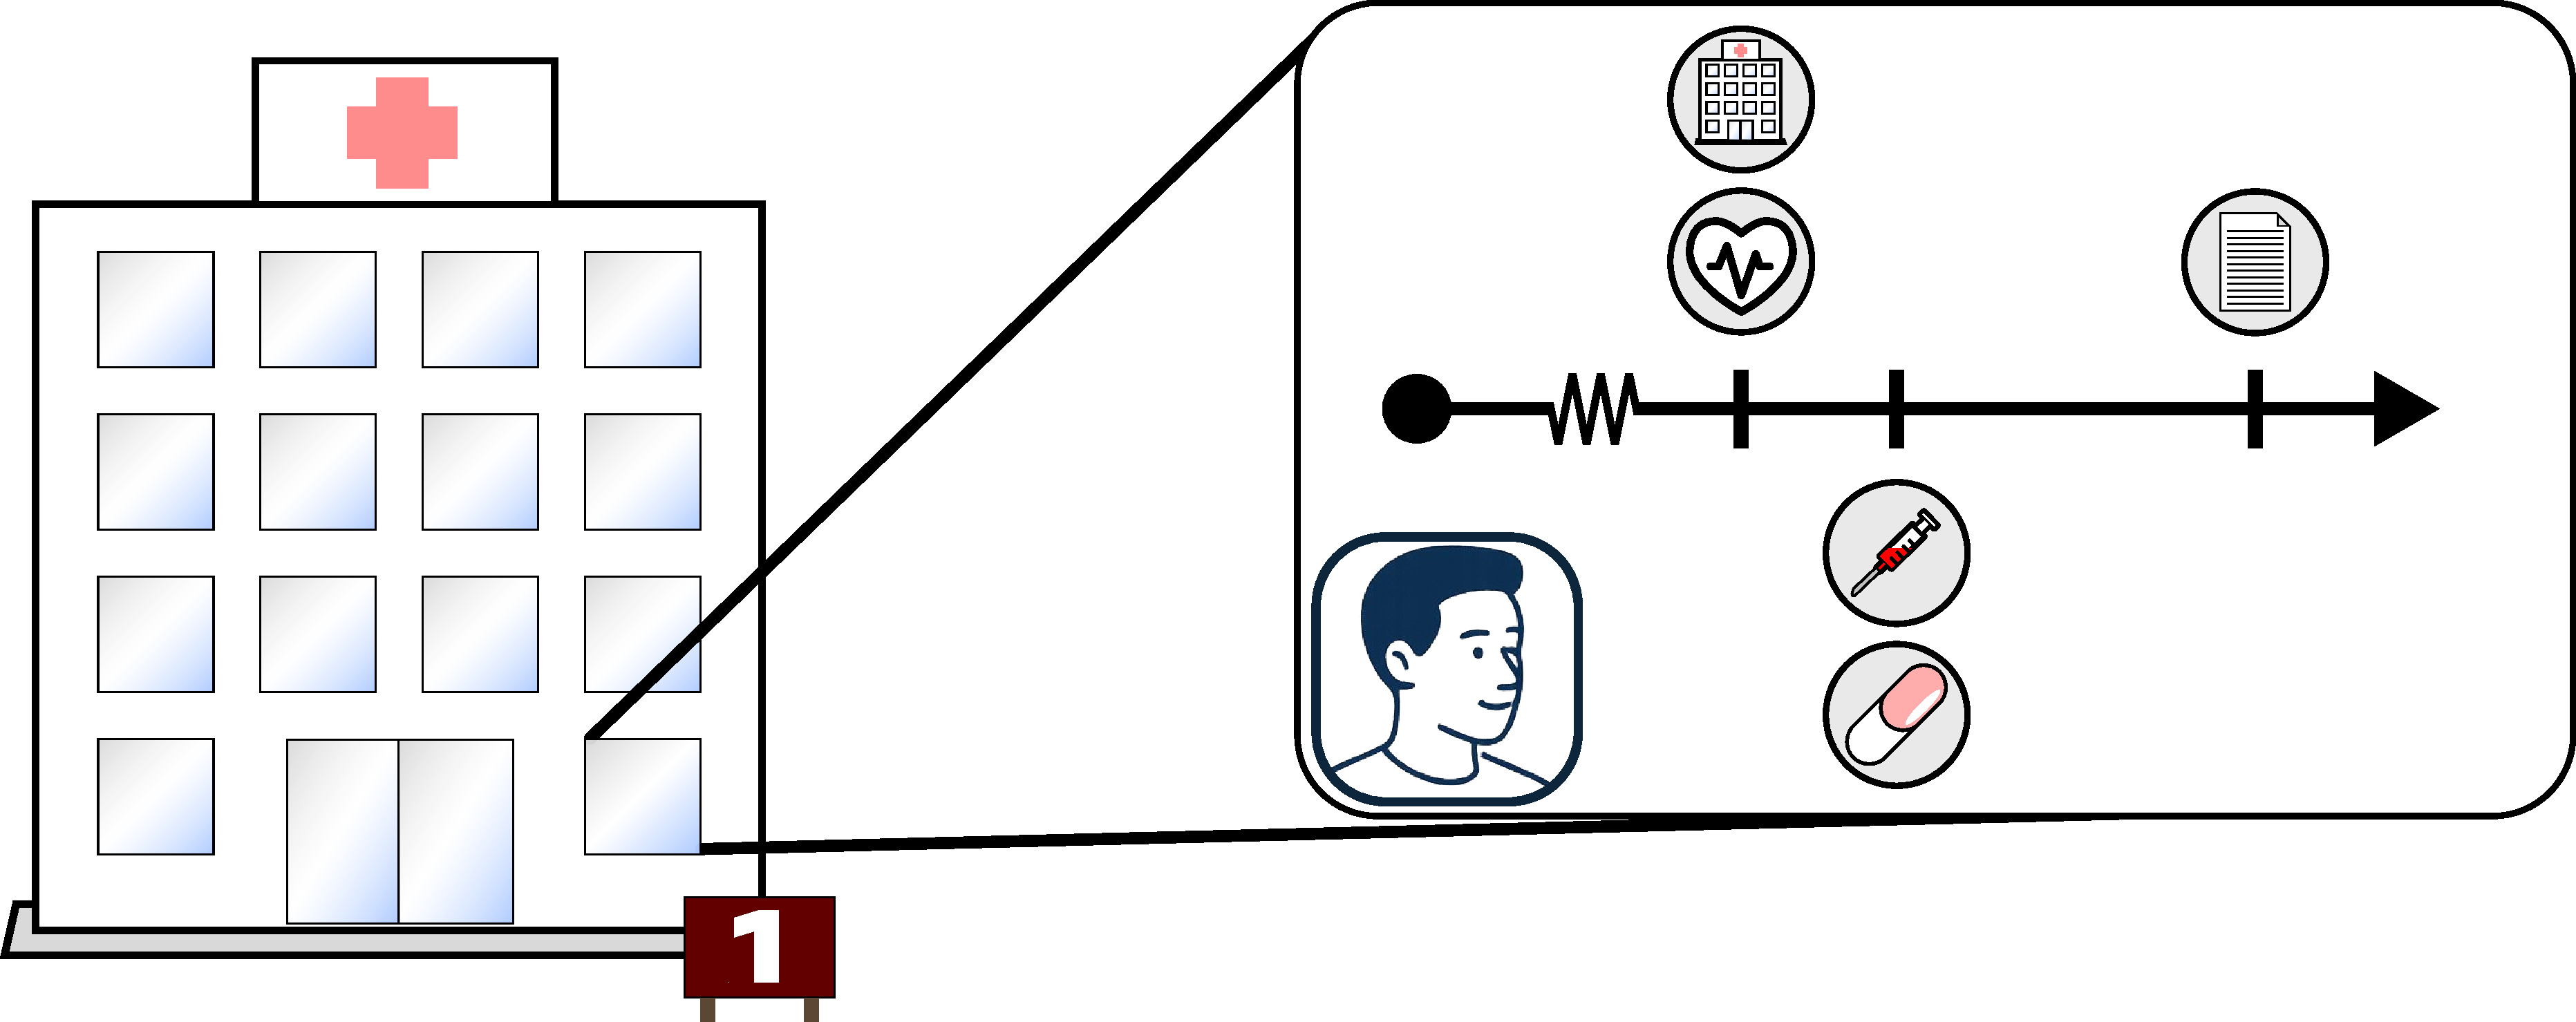
\includegraphics[width=0.75\linewidth,height=0.40\textheight,keepaspectratio]{figures/fig19_timeline_with_note.pdf}
\end{center}

\vspace{-0.2em}
\small
A clinical note is never standalone. It sits in a \textbf{longitudinal sequence} --- referencing prior notes, labs, imaging, and medication orders.

\pause
\vspace{0.1em}
Copy-paste across visits is why the i.i.d.\ assumption fails. The COMPARISON line in radiology reports is an explicit temporal link. And notes reference images and labs that aren't in the text at all --- \textbf{multi-modal linkage} that a text-only model will miss.
\end{frame}

% ============================================================
\begin{frame}{Abbreviations}
\textbf{Abbreviations} are pervasive and ambiguous:

\vspace{0.2em}
\begin{center}
\small
\begin{tabular}{ll}
\toprule
\textbf{Abbrev.} & \textbf{Possible meanings} \\
\midrule
MS & Multiple sclerosis, mitral stenosis, morphine sulfate, mental status, \ldots \\
CP & Chest pain, cerebral palsy, cleft palate \\
PE & Pulmonary embolism, physical exam, pleural effusion \\
\bottomrule
\end{tabular}
\end{center}

\vspace{0.15em}
Disambiguation requires \emph{context}: the same abbreviation means different things in a cardiology note vs.\ a neurology note vs.\ a pharmacy order.

\pause
\datatypebox{Tokens are nominal, but their meaning depends on \textbf{section structure}. ``ROS'' vs.\ ``Assessment'' headers change what ``MS'' means --- positional context within the note is semantic, not just sequential.}
\end{frame}

% ============================================================
\begin{frame}{How Ambiguous Are Clinical Abbreviations?}
\begin{center}
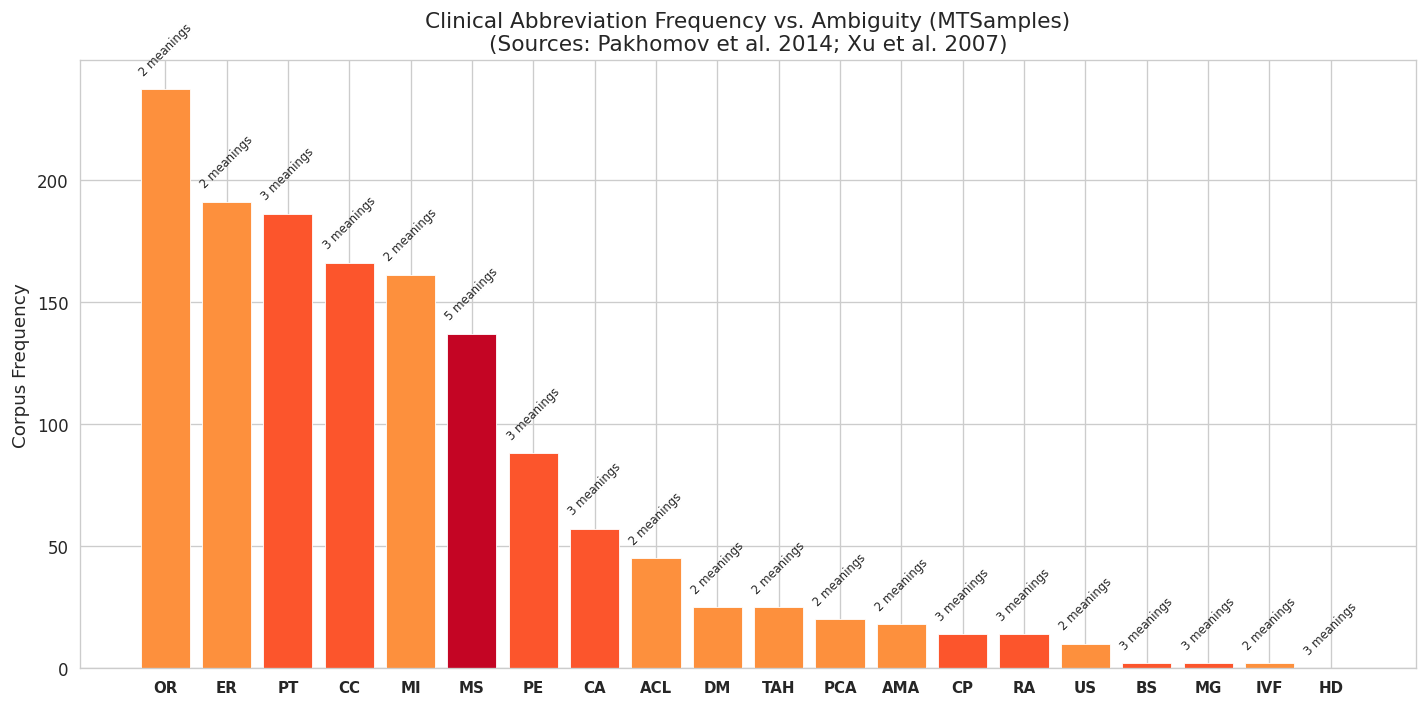
\includegraphics[width=0.88\linewidth,height=0.65\textheight,keepaspectratio]{figures/fig19_4_abbreviation_ambiguity.png}
\end{center}

\vspace{-0.3em}
\small
Frequency vs.\ number of meanings for 20 abbreviations validated against Pakhomov et al.\ (2014) and Xu et al.\ (2007). {\footnotesize [Notebook Cell~7]}
\end{frame}

% ============================================================
\begin{frame}{Negation in Clinical Text}
``No evidence of malignancy'' \emph{contains} the word ``malignancy'' --- a bag-of-words model treats this as evidence \emph{for} cancer.

\pause
\vspace{0.2em}
\textbf{Why is this so common in clinical text?} Clinicians document by \emph{exclusion}: the Review of Systems lists everything the patient \emph{denies}. Studies on real EHR data report \textbf{30--50\% of medical concepts negated} (Chapman et al., 2001; Harkema et al., 2009). Our MTSamples analysis shows similar patterns.

\pause
\vspace{0.2em}
Dedicated clinical negation tools (NegEx, ConText, NegBio) exist precisely because general-purpose NLP methods underperform at this density.

\vspace{0.1em}
{\footnotesize \textbf{Note:} Negation isn't unique to clinical text --- sentiment analysis (``not bad'') and legal text (``no liability'') face it too. But the \emph{rate} is far higher in clinical notes than in any general-domain corpus.}
\end{frame}

% ============================================================
\begin{frame}{How Much Negation? Prevalence by Condition}
\begin{center}
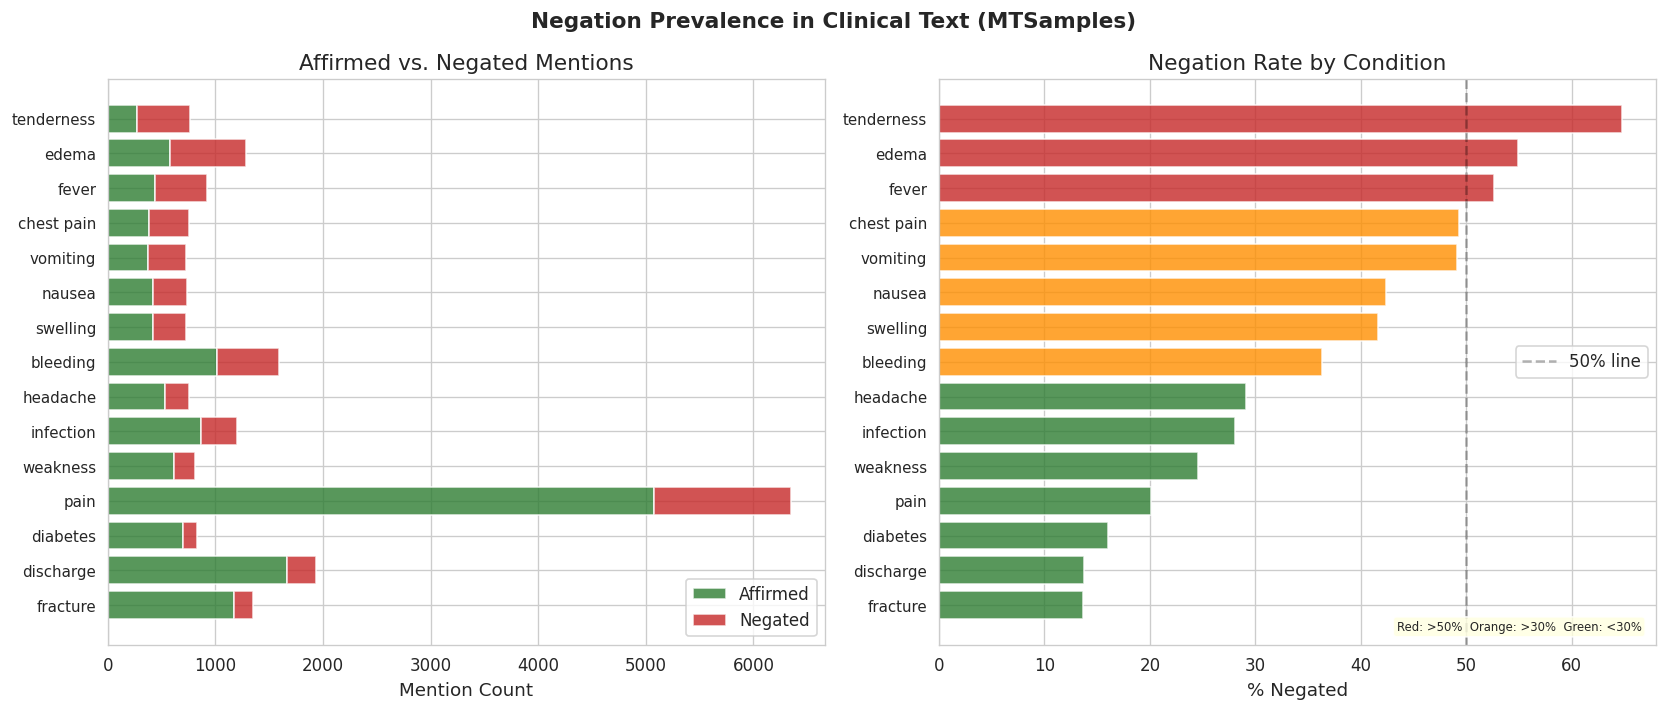
\includegraphics[width=0.88\linewidth,height=0.66\textheight,keepaspectratio]{figures/fig19_5_negation_prevalence.png}
\end{center}

\vspace{-0.3em}
\small
Rash and tenderness are negated $>$60\% of the time --- a keyword model would invert their meaning. {\footnotesize [Notebook Cell~8]}
\end{frame}

% ============================================================
\section{Clinical Communication}

% ============================================================
\begin{frame}{Text Written for Other Clinicians}
Some clinical text is primarily \textbf{communicative} --- written by one clinician for another:

\vspace{0.1em}
\textbf{Radiology / pathology reports:} A specialist interprets a study and communicates findings to the ordering provider.
\begin{itemize}[<+->]\setlength\itemsep{0.02em}
  \item Semi-structured: Indication, Technique, Findings, Impression.
  \item One report = one study/specimen (not an evolving narrative like progress notes).
  \item Impression section is the ``answer'' --- often used as \textbf{silver-standard labels} for imaging ML (e.g., CheXpert extracts labels from report text).
\end{itemize}

\onslide<4->{\textbf{Consult notes, referral letters:} One specialist writes to another. More structured than progress notes.

\vspace{0.05em}
\alert{Key difference from documentation:} Less copy-paste, more targeted communication. But still templated and billing-driven.}
\end{frame}

% ============================================================
\begin{frame}{Example: A Radiology Report}
\begin{columns}[T]
\begin{column}{0.50\textwidth}
\scriptsize
\texttt{\textbf{INDICATION:} 45F, cough, fever, r/o PNA.}\\[1pt]
\texttt{\textbf{TECHNIQUE:} PA and lateral CXR.}\\[1pt]
\texttt{\textbf{COMPARISON:} Prior 2025-12-01.}\\[1pt]
\texttt{\textbf{FINDINGS:} Heart size normal. Lungs clear bilat. No consolidation, effusion, or PTX. Osseous structures intact.}\\[1pt]
\texttt{\textbf{IMPRESSION:} No acute cardiopulmonary abnormality.}
\end{column}
\begin{column}{0.47\textwidth}
\footnotesize
\begin{itemize}[<+->]\setlength\itemsep{0.01em}
  \item \textbf{Rigid section structure} --- far more than progress notes.
  \item \textbf{Less copy-paste}, but heavy template use (normals are boilerplate).
  \item \textbf{COMPARISON line} = explicit temporal link to prior imaging.
  \item High negation: ``No consolidation, no effusion\ldots''
\end{itemize}
\end{column}
\end{columns}

\onslide<5->{\datatypebox{Three data-type issues in one report: \textbf{(1)} section headers change token semantics, \textbf{(2)} COMPARISON line encodes \textbf{temporal} dependence, \textbf{(3)} the report \textbf{references an image} --- text alone is incomplete (\textbf{multi-modal linkage}).}}
\end{frame}

% ============================================================
\begin{frame}{Text Written for Patients}
\small
A growing category, especially post-21st Century Cures Act (2021), which gave patients access to their own notes (``OpenNotes'').

\vspace{0.1em}
\textbf{After-visit summaries (AVS):} Auto-generated plain-language summaries given to patients after an encounter.

\vspace{0.1em}
\textbf{Patient-facing letters:} LLMs are increasingly used to draft replies to portal messages, lab result explanations, post-discharge instructions.

\pause
\vspace{0.1em}
\textbf{The tension:} Clinical documentation has historically been clinician-to-clinician jargon. Now patients are reading it --- pressure to simplify risks watering down clinical specificity.

\pause
\vspace{0.1em}
\alert{Privacy \& de-identification:} HIPAA's 18 identifiers must be removed before research use. De-id tools replace PHI with tokens like \texttt{[DATE]}, \texttt{[NAME]} --- these artifacts become part of your data distribution.
\end{frame}

% ============================================================
\section{Patient-Generated Text}

% ============================================================
\begin{frame}{Patient-Generated Text}
A rapidly growing source of health text that doesn't come from clinicians:

\vspace{0.15em}
\begin{itemize}[<+->]\setlength\itemsep{0.02em}
  \item \textbf{Patient portal messages:} Direct messages to providers via MyChart, etc. Informal, varied literacy levels, often the first signal of a problem.
  \item \textbf{Social media:} Reddit (r/AskDocs, disease-specific subs), Twitter/X, patient forums (PatientsLikeMe). Useful for pharmacovigilance, disease surveillance.
  \item \textbf{Online health communities:} WebMD, HealthUnlocked. Vernacular differs from clinical terminology (``dizzy'' vs.\ ``vertigo''; ``can't breathe'' vs.\ ``dyspnea'').
\end{itemize}

\onslide<4->{\textbf{Key challenge:} The vocabulary gap. Patients and clinicians describe the same conditions using different words. Models trained on clinical text may fail on patient text, and vice versa.}
\end{frame}

% ============================================================
\section{Scientific \& Biomedical Literature}

% ============================================================
\begin{frame}{Biomedical Literature}
\small
\textbf{PubMed:} 36M+ abstracts. \textbf{PMC:} Full-text open-access subset. Fundamentally different from clinical text:

\vspace{0.05em}
\begin{center}
\scriptsize
\begin{tabular}{lcc}
\toprule
\textbf{Property} & \textbf{Clinical Notes} & \textbf{PubMed} \\
\midrule
Purpose & Documentation / billing & Knowledge dissemination \\
Author & Clinician (time-pressured) & Researcher (edited, reviewed) \\
Vocabulary & Abbreviations, slang & Formal terminology \\
PHI? & Yes & No \\
Temporal? & Yes (longitudinal) & No (standalone articles) \\
\bottomrule
\end{tabular}
\end{center}

\pause
\vspace{0.05em}
\textbf{Controlled vocabularies:} Papers aren't \emph{written in} controlled vocabularies --- they use many of the same terms. \textbf{MeSH} is \emph{metadata}: NLM indexers tag articles with MeSH headings \emph{after} publication. \textbf{UMLS} links terminologies (ICD, SNOMED, MeSH) into a metathesaurus.
\end{frame}

% ============================================================
\begin{frame}{What Does Each Text Type Actually Look Like?}
\scriptsize
\begin{columns}[T]
\begin{column}{0.48\textwidth}
\colorbox{accentOrange!8}{\parbox{\dimexpr\linewidth-2\fboxsep}{\textbf{Clinical Note}\\[2pt]
\texttt{63M w/ h/o HTN, DM2, CKD3 p/w AMS. Pt found down at home, GCS 11. Labs: Cr 4.2 (baseline 2.1), K 6.1. A\&P: AKI on CKD, likely prerenal 2/2 dehydration. IVF NS @ 150cc/hr.}
}}

\vspace{0.2em}
\colorbox{columbiaBlue!8}{\parbox{\dimexpr\linewidth-2\fboxsep}{\textbf{PubMed Abstract}\\[2pt]
\texttt{BACKGROUND: Acute kidney injury (AKI) complicates 10--15\% of hospital admissions and is associated with increased mortality. METHODS: We conducted a retrospective cohort study of 12,413 patients\ldots}
}}
\end{column}
\begin{column}{0.48\textwidth}
\colorbox{codeGreen!8}{\parbox{\dimexpr\linewidth-2\fboxsep}{\textbf{Patient Portal Message}\\[2pt]
\texttt{Hi Dr. Smith, I got my blood work back and my creatinine is 4.2 which seems really high?? I've been feeling tired and not eating much. Should I go to the ER or wait until Thursday?}
}}

\vspace{0.2em}
\colorbox{lightGray}{\parbox{\dimexpr\linewidth-2\fboxsep}{\textbf{Medical Textbook}\\[2pt]
\texttt{Acute kidney injury is defined as an abrupt decrease in renal function, resulting in retention of urea and other nitrogenous waste products. The KDIGO criteria classify AKI into three stages\ldots}
}}
\end{column}
\end{columns}

\normalsize
\vspace{0.15em}
\alert{Same clinical situation, four texts.} Notice abbreviation density, formality, and assumed reader knowledge. {\footnotesize [Notebook Cell~10]}
\end{frame}

% ============================================================
\begin{frame}{The Vocabulary Gap Across Domains}
\begin{center}
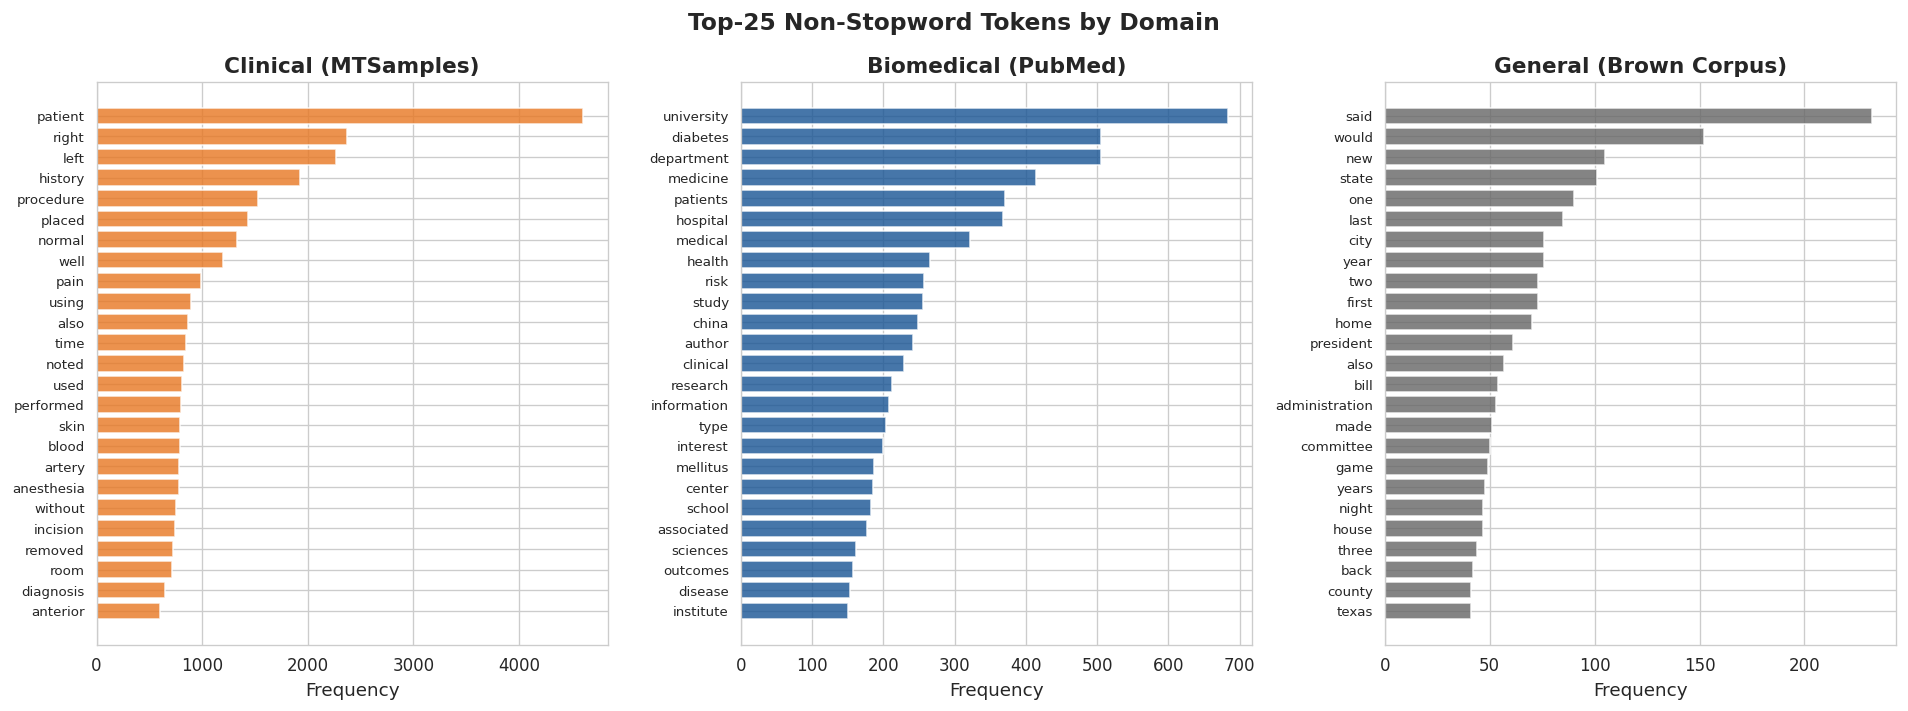
\includegraphics[width=0.92\linewidth,height=0.66\textheight,keepaspectratio]{figures/fig19_2_vocab_comparison.png}
\end{center}

\vspace{-0.3em}
\small
Top-25 non-stopword tokens from clinical notes, PubMed abstracts, and general English. Almost zero overlap --- a model trained on one domain will struggle with the others. {\footnotesize [Notebook Cell~5]}
\end{frame}

% ============================================================
\begin{frame}{How Does Biomedical Text Differ from Other Academic Text?}
Why not just use a general-domain language model trained on all of academia?

\vspace{0.2em}
\begin{itemize}[<+->]\setlength\itemsep{0.05em}
  \item \textbf{Dense specialized vocabulary.} More named entities per sentence (genes, proteins, drugs, diseases) than most fields. ``p53'' is unambiguous in biology, opaque elsewhere.
  \item \textbf{Structured abstracts.} Background / Methods / Results / Conclusion format is near-universal in clinical journals --- rare in CS, humanities, social science.
  \item \textbf{Massive scale.} PubMed is $>$36M articles; arXiv is $\sim$2.5M.
  \item \textbf{Direct clinical relevance.} Findings may affect patient care --- factuality stakes are higher than in most academic domains.
\end{itemize}

\onslide<5->{This is why domain-specific models (PubMedBERT, BioGPT, SciBERT) consistently outperform general models on biomedical benchmarks.}
\end{frame}

% ============================================================
\begin{frame}{Datasets \& Gotchas}
\begin{columns}[T]
\begin{column}{0.57\textwidth}
\scriptsize
\textbf{Where do researchers get health text data?}
\begin{itemize}\setlength\itemsep{0.0em}
  \item \textbf{MIMIC-III/IV}: De-identified ICU notes, credentialed access. Most-used clinical NLP dataset --- but skewed toward critical illness.
  \item \textbf{MTSamples}: Open-access transcribed reports. Small, noisy, no longitudinal patient structure.
  \item \textbf{PubMed / PMC}: Open. Indexes broadly --- vet science, traditional medicine, predatory journals, retracted papers mixed in.
  \item \textbf{MIMIC-CXR}: Radiology reports + chest X-rays. Silver labels from text.
\end{itemize}
\end{column}
\begin{column}{0.41\textwidth}
\centering
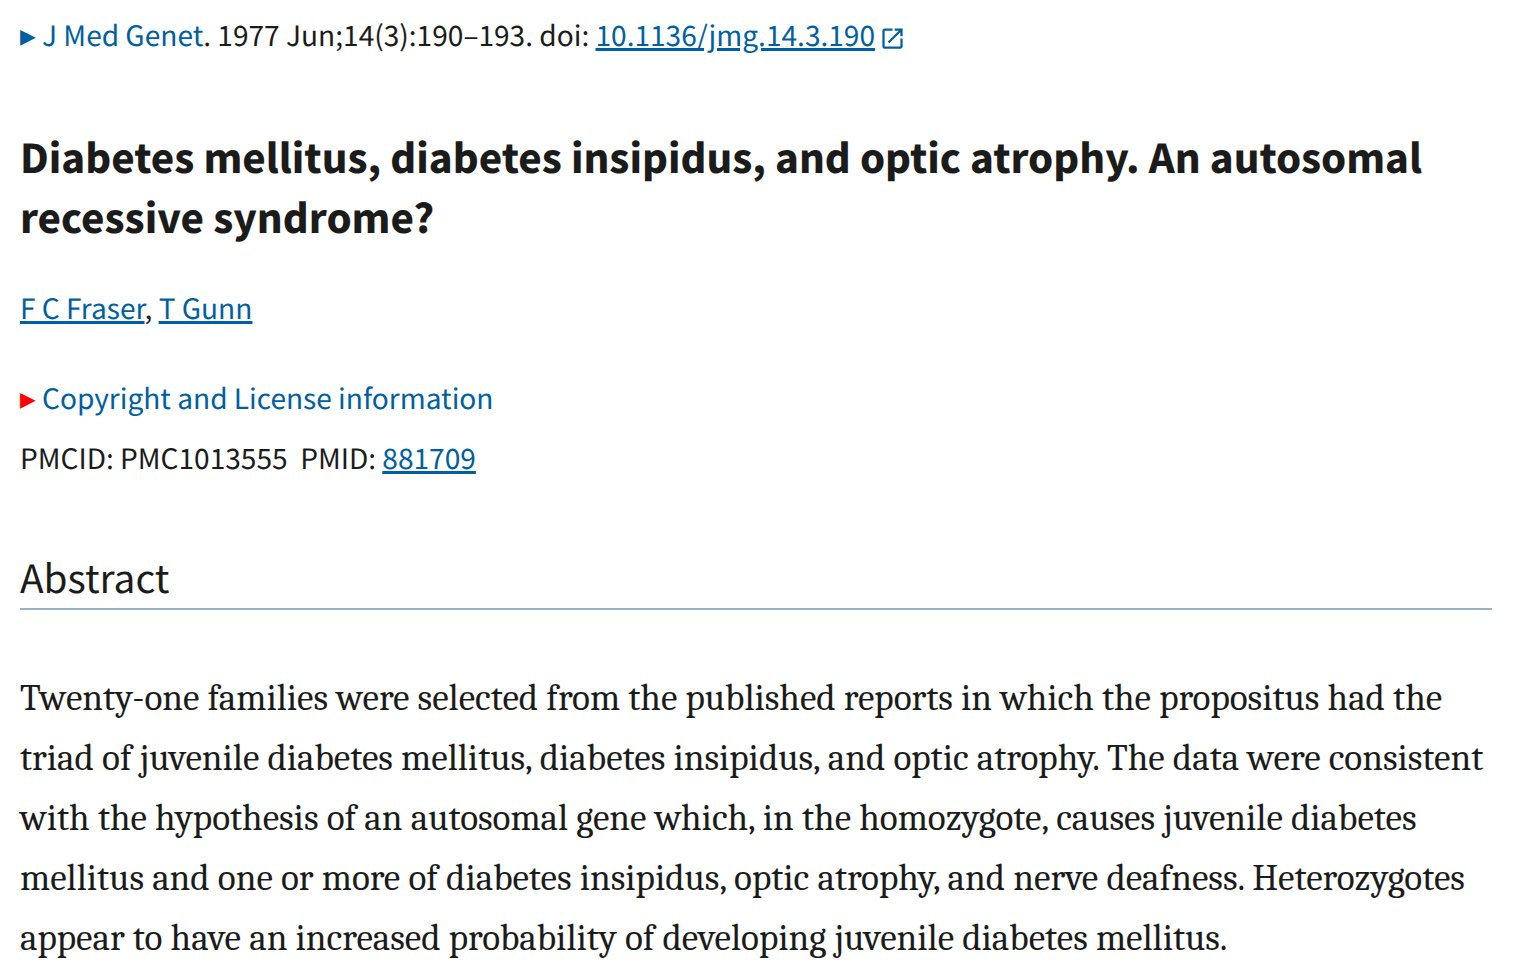
\includegraphics[width=\linewidth,height=3.2cm,keepaspectratio]{figures/fig19_pubmed_case_report.png}\\[1pt]
{\scriptsize A 1977 case report on a rare syndrome --- published \emph{because} it's unusual.}
\end{column}
\end{columns}

\vspace{0.05em}
\small
\textbf{Horses vs.\ zebras:} Clinical notes are dominated by common conditions. PubMed \textbf{case reports} overrepresent rare findings --- they invert the base-rate distribution.
\alert{Know your data source's selection bias before you train on it.}
\end{frame}

% ============================================================
\section{How Text is Changing Right Now}

% ============================================================
\begin{frame}{Ambient AI Scribes: The Biggest Shift in Clinical Documentation}
\textbf{Ambient AI scribes} (Nuance DAX Copilot, Abridge, Suki, etc.) listen to patient--provider conversations and auto-generate structured clinical notes.

\vspace{0.3em}
\textbf{What we know so far:}
\begin{itemize}[<+->]\setlength\itemsep{0.1em}
  \item Physicians report saving 1--3 hours/day on documentation.
  \item Burnout reduction: one study saw rates drop from 52\% to 39\% (Shah et al., 2025).
  \item The VA has deployed ambient scribes system-wide.
  \item Note quality is generally acceptable, with $\sim$1.5\% hallucination rate (Asgari et al., 2025).
\end{itemize}
\end{frame}

% ============================================================
\begin{frame}{Ambient AI Scribes: The Catch}
The promise is ``less documentation burden.'' The reality is more nuanced:

\vspace{0.2em}
\begin{itemize}[<+->]\setlength\itemsep{0.08em}
  \item Notes become \emph{longer and more detailed} --- not shorter.
  \item The business case is shifting from ``save time'' to ``\textbf{capture more revenue}'' through more thorough coding documentation.
  \item Insurers are already responding with automated downcoding.
  \item Scribe-generated notes have \textbf{different statistical properties}: more fluent, fewer abbreviations, more uniform structure --- models trained on human-written notes may not transfer.
\end{itemize}

\onslide<5->{\datatypebox{The \textbf{generative origin} of clinical text is changing. Yesterday's training data was human-written under time pressure; tomorrow's is LLM-generated under revenue pressure. Same token vocabulary, different distribution.}}
\end{frame}

% ============================================================
\begin{frame}{The Jevons Paradox of Clinical Documentation}
\textbf{Recall the paradox} from the start of lecture.

\vspace{0.2em}
\small
\begin{enumerate}[<+->]\setlength\itemsep{0.1em}
  \item \textbf{1990s--2000s:} EHR templates designed to make documentation \emph{faster}.
  $\Rightarrow$ Notes got \emph{longer} (copy-paste, template proliferation).

  \item \textbf{2010s:} Coding requirements incentivized \emph{thorough} documentation.
  $\Rightarrow$ Even more boilerplate. Information per word \emph{decreased}.

  \item \textbf{2020s:} Ambient AI scribes make documentation essentially \emph{free}.
  $\Rightarrow$ Notes are \emph{even longer}. Revenue optimization kicks in.
\end{enumerate}
\normalsize

\onslide<4->{
\vspace{0.2em}
\textbf{The pattern:} Making documentation easier has increased text volume while \emph{decreasing} information density at each step.

\vspace{0.1em}
\alert{For ML researchers:} The statistical properties of clinical text are a \emph{moving target}.}
\end{frame}

% ============================================================
\begin{frame}{LLMs Are Also Changing the \emph{Reading} Side}
It's not just writing --- LLMs are increasingly used to \emph{process} clinical text:

\vspace{0.15em}
\begin{itemize}[<+->]\setlength\itemsep{0.02em}
  \item \textbf{Patient message triage:} LLMs classify portal messages by urgency.
  \item \textbf{After-visit summaries:} LLMs generate plain-language summaries of encounters.
  \item \textbf{Lab result explanations:} LLMs draft patient-facing explanations of results.
  \item \textbf{Prior authorization:} LLMs draft letters justifying treatments to insurers.
  \item \textbf{Literature search:} LLMs summarize PubMed results for clinical questions.
\end{itemize}

\onslide<6->{\textbf{The implication:} We are entering a world where LLMs both \emph{write} and \emph{read} clinical text. The human may be out of the loop in both directions. This raises fundamental questions about \textbf{factuality}, \textbf{accountability}, and \textbf{drift}.}
\end{frame}

% ============================================================
\section{Bringing It Together}

% ============================================================
\begin{frame}{Five Ways Clinical Text Breaks the ``Sequence of Tokens'' Abstraction}
\small
Text is a \emph{sequence of nominal tokens} --- but today we saw five ways this breaks down:

\vspace{0.05em}
\begin{center}
\scriptsize
\renewcommand{\arraystretch}{1.0}
\begin{tabular}{@{}p{2.2cm}p{4.0cm}p{3.6cm}@{}}
\toprule
\textbf{Issue} & \textbf{Where we saw it} & \textbf{ML consequence} \\
\midrule
Section structure & ``MS'' means different things in ROS vs.\ A\&P; rigid rad report sections & BoW fails; need section-aware features \\
Temporal dependence & Copy-paste across visits; rad COMPARISON line & Split by patient, not note \\
Multi-modal links & Reports reference images, labs, orders & Text alone is incomplete \\
i.i.d.\ violation & 50--80\% duplication (heatmap) & Train--test leakage \\
Generative origin shift & AI scribes changing note statistics & Distribution drift \\
\bottomrule
\end{tabular}
\end{center}
\vspace{-0.1em}
\alert{Bottom line:} Clinical text \emph{looks like} a standard NLP problem. The pathologies above are why it isn't.
\end{frame}

% ============================================================
\section{Wrap-up}

% ============================================================
\begin{frame}{Key Takeaways}
\begin{enumerate}[<+->]\setlength\itemsep{0.02em}
  \item Health text comes in many forms. The key organizing principle is \textbf{who writes, for whom, and why}.
  \item Clinical documentation is driven by \textbf{billing and legal requirements} under time pressure --- templates, copy-paste, and abbreviations are rational coping strategies.
  \item Much clinical ``text'' is \textbf{machine-generated boilerplate} --- an LLM trained on it is partly learning to emulate template engines, not human communication.
  \item \textbf{The Jevons Paradox}: each documentation technology wave has increased text volume while decreasing information density.
  \item The vocabulary gap between clinical, scientific, and patient text means \textbf{domain adaptation is essential}. Know your dataset's selection bias.
\end{enumerate}

\onslide<6->{\alert{Thursday:} How do we \emph{model} all of this? Domain adaptation, fairness in clinical NLP, factuality, and evidence-grounded generation.}
\end{frame}

% ============================================================
\begin{frame}{References \& Further Reading}
\tiny
\begin{columns}[T]
\begin{column}{0.48\textwidth}
\textbf{Documentation burden \& clinical text:}\\
Sinsky et al.\ (2016). \emph{Allocation of physician time.} Ann Intern Med.\\
Tsou et al.\ (2017). \emph{Copy-paste prevalence.} JAMA Intern Med.\\
Cohen et al.\ (2013). \emph{Copy-paste note bloat.} IJMI.

\vspace{0.1em}
\textbf{Negation \& abbreviation disambiguation:}\\
Chapman et al.\ (2001). \emph{NegEx.} AMIA.\\
Harkema et al.\ (2009). \emph{ConText.} JBI.\\
Pakhomov et al.\ (2014). \emph{Clinical abbreviation sense inventory.} JAMIA.\\
Xu et al.\ (2007). \emph{Sense inventory methods.} AMIA.

\vspace{0.1em}
\textbf{Ambient AI scribes:}\\
Shah et al.\ (2025). \emph{Burnout and ambient AI documentation.}\\
Asgari et al.\ (2025). \emph{Hallucination rates in AI-generated notes.}
\end{column}
\begin{column}{0.48\textwidth}
\textbf{Also referenced:}\\
Irvin et al.\ (2019). \emph{CheXpert.} AAAI.\\
21st Century Cures Act (2016/2021): OpenNotes.\\
Jevons, W.S.\ (1865). \emph{The Coal Question.}

\vspace{0.1em}
\textbf{Datasets:}\\
MIMIC-III/IV: \texttt{physionet.org}\\
MTSamples: \texttt{kaggle.com}\\
PubMed/PMC: \texttt{pubmed.ncbi.nlm.nih.gov}\\
MedRAG corpora: \texttt{huggingface.co/MedRAG}\\
ChatDoctor: \texttt{huggingface.co/datasets/avaliev/chat\_doctor}
\end{column}
\end{columns}
\end{frame}

% ============================================================
\begin{frame}[standout]
  Questions?\\[1em]
  {\small Next: Lecture 20 --- Clinical \& Biomedical NLP: Modeling}
\end{frame}

\end{document}